\documentclass[aspectratio=169, 10pt]{beamer}

\usepackage[T1]{fontenc}
\usepackage[utf8]{inputenc}
\usepackage{lmodern}
\usepackage{amsmath, amssymb}
\usepackage{booktabs}
\usepackage[table]{xcolor}
\usepackage{bookmark}
\usepackage{tikz}
\usetikzlibrary{arrows.meta, positioning}

% --- Theme & Palette ---
\usetheme[progressbar=frametitle, numbering=fraction, block=fill, sectionpage=none]{metropolis}

\definecolor{PrimaryTeal}{HTML}{0b5313}
\definecolor{AccentTerra}{HTML}{C85A32}
\definecolor{SoftSlate}{HTML}{52606D}
\definecolor{BgLight}{HTML}{FAFAFA}
\definecolor{CardFill}{HTML}{EEF3F5}

\setbeamercolor{background canvas}{bg=BgLight}
\setbeamercolor{palette primary}{bg=PrimaryTeal, fg=white}
\setbeamercolor{frametitle}{bg=PrimaryTeal, fg=white}
\setbeamercolor{title separator}{fg=AccentTerra}
\setbeamercolor{progress bar}{fg=AccentTerra, bg=CardFill}
\setbeamercolor{alerted text}{fg=AccentTerra}
\setbeamercolor{block title}{bg=PrimaryTeal, fg=white}
\setbeamercolor{block body}{bg=CardFill, fg=PrimaryTeal}
\setbeamercolor{block title alerted}{bg=AccentTerra, fg=white}
\setbeamercolor{block body alerted}{bg=CardFill, fg=PrimaryTeal}

\setbeamerfont{title}{size=\Large, series=\bfseries}
\setbeamerfont{subtitle}{size=\normalsize}
\setbeamerfont{frametitle}{size=\normalsize, series=\bfseries}

\title{Can Language Create Cooperation?}
\subtitle{Natural-Language Negotiation in Strategic Multi-Agent LLM Interactions}
\author{Gabriele Granzotto}
\institute{University of Trieste --- Multi-Agent Systems}
\date{\resizebox{0.88\textwidth}{!}{\texttt{\url{https://github.com/GabrieleGranzotto/Multi-Agent-Language-Model-Cooperation-Analysis}}}}

\begin{document}

% ==============================================================================
% SLIDE 1: Title
% ==============================================================================
\begin{frame}[plain]
    \titlepage
\end{frame}

% ==============================================================================
% SECTION 1: Strategic Setting & Architecture
% ==============================================================================
\section{Strategic Setting \& System Architecture}

% SLIDE 2: Motivation & Controlled Ablation Design
\begin{frame}{Motivation \& Controlled Experimental Design}
    \small
    \begin{columns}[T, totalwidth=\textwidth]
        \begin{column}{0.52\textwidth}
            \begin{block}{Research Question}
                Can non-binding pre-play communication (\emph{cheap talk}) induce emergent cooperation between autonomous LLM agents in a one-shot social dilemma where strict rationality dictates defection?
            \end{block}
            \vspace{0.2cm}
            \begin{itemize}
                \setlength{\itemsep}{5pt}
                \item \textbf{Game-Theoretic Baseline:} Without binding commitments, cheap talk is costless and cannot alter Nash equilibria.
                \item \textbf{LLM Strategic Reasoning:} Language models condition choices on verbal trust signals and joint-welfare framing.
                \item \textbf{Causal Isolation:} A $0$-turn silent baseline separates static RLHF alignment bias from genuine negotiation effects.
            \end{itemize}
        \end{column}
        \begin{column}{0.44\textwidth}
            \begin{alertblock}{Experimental Setup}
                \begin{itemize}
                    \setlength{\itemsep}{6pt}
                    \item \textbf{Model Backend:} Local \texttt{gemma4} via \texttt{Ollama} (homogeneous symmetric self-play).
                    \item \textbf{Baseline ($0$ Turns):} $N = 200$ matches ($400$ decisions) with simultaneous silent choice.
                    \item \textbf{Negotiation (Chat):} $N = 300$ matches ($600$ decisions) with alternating natural-language turns.
                    \item \textbf{Randomization:} First speaker (\emph{Initiator} vs. \emph{Responder}) sampled uniformly.
                \end{itemize}
            \end{alertblock}
        \end{column}
    \end{columns}
\end{frame}

% SLIDE 3: Game-Theoretic Formulation
\begin{frame}{Game-Theoretic Formulation: Prisoner's Dilemma}
    \small
    \begin{columns}[T, totalwidth=\textwidth]
        \begin{column}{0.52\textwidth}
            \textbf{Normal-Form Game:} $G = (N, A, u)$ with $N = \{A, B\}$, $A = \prod_{i \in N} A_i$, $A_i = \{\text{Cooperate}, \text{Defect}\}$, and $u: A \to \mathbb{R}^N$.
            \vspace{0.2cm}
            \begin{itemize}
                \setlength{\itemsep}{6pt}
                \item \textbf{Nash Equilibrium ($s^* \in A$):} No player can unilaterally deviate and improve payoff:
                      \[
                          u_i(s^*) \ge u_i(s_i, s_{-i}^*) \quad \forall i \in N,\; \forall s_i \in A_i.
                      \]
                \item \textbf{Pareto Optimal Outcome ($s^* \in A$):} No $s' \in A$ satisfies $u_i(s') \ge u_i(s^*)$ for all $i \in N$ with strict inequality for at least one $j \in N$.
            \end{itemize}
        \end{column}
        \begin{column}{0.44\textwidth}
            \centering
            \textbf{Payoff Matrix $(u_A, u_B)$}
            \vspace{0.2cm}
            \begin{tabular}{lcc}
                \toprule
                \textbf{Agent A / Agent B} & \textbf{Cooperate (C)} & \textbf{Defect (D)} \\
                \midrule
                \textbf{Cooperate (C)}     & $(3, 3)$               & $(0, 5)$            \\
                \textbf{Defect (D)}        & $(5, 0)$               & $(1, 1)$            \\
                \bottomrule
            \end{tabular}
            \vspace{0.3cm}
            \begin{block}{Strategic Tension}
                Since $T=5 > R=3 > P=1 > S=0$, mutual defection $(D,D)$ is the unique strictly dominant Nash Equilibrium (welfare $= 2$), whereas $(C,C)$ is Pareto optimal (welfare $= 6$).
            \end{block}
        \end{column}
    \end{columns}
\end{frame}

% SLIDE 4: Three-Phase Interaction Protocol
\begin{frame}{System Architecture \& Three-Phase Protocol}
    \small
    \centering
    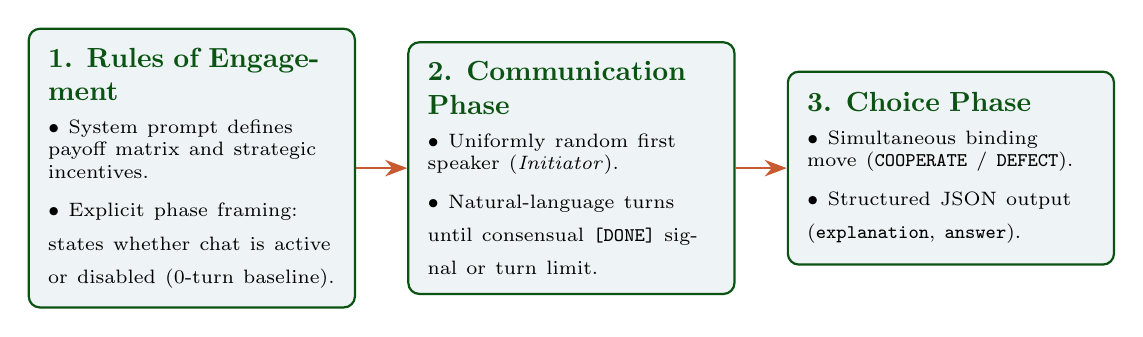
\begin{tikzpicture}[
        phase/.style={draw=PrimaryTeal, thick, rounded corners=4pt, fill=CardFill, text width=3.65cm, minimum height=2.45cm, align=left, inner sep=7pt},
        arrow/.style={-{Stealth[length=2.8mm]}, thick, color=AccentTerra}
        ]
        \node[phase] (p1) at (0,0) {
            \textbf{\color{PrimaryTeal}1. Rules of Engagement}\\[4pt]
            \scriptsize
            $\bullet$ System prompt defines payoff matrix and strategic incentives.\\[2pt]
            $\bullet$ Explicit phase framing: states whether chat is active or disabled ($0$-turn baseline).
        };
        \node[phase, right=0.65cm of p1] (p2) {
            \textbf{\color{PrimaryTeal}2. Communication Phase}\\[4pt]
            \scriptsize
            $\bullet$ Uniformly random first speaker (\emph{Initiator}).\\[2pt]
            $\bullet$ Natural-language turns until consensual \texttt{[DONE]} signal or turn limit.
        };
        \node[phase, right=0.65cm of p2] (p3) {
            \textbf{\color{PrimaryTeal}3. Choice Phase}\\[4pt]
            \scriptsize
            $\bullet$ Simultaneous binding move (\texttt{COOPERATE} / \texttt{DEFECT}).\\[2pt]
            $\bullet$ Structured JSON output (\texttt{explanation}, \texttt{answer}).
        };
        \draw[arrow] (p1.east) -- (p2.west);
        \draw[arrow] (p2.east) -- (p3.west);
    \end{tikzpicture}
    \vspace{0.3cm}
    \begin{block}{Automated Reproducibility \& Analytics Pipeline}
        Every run logs full transcripts, sanity-check telemetry, and structured JSON decisions (\textbf{0.0\% parsing error rate}), automatically exporting non-parametric tests, HTML conversation reports, and map-reduce explanation syntheses.
    \end{block}
\end{frame}

% SLIDE 5: Alignment Safeguards & Sanity-Check Pipeline
\begin{frame}{Alignment Safeguards \& Sanity-Check Telemetry}
    \small
    \begin{columns}[T, totalwidth=\textwidth]
        \begin{column}{0.40\textwidth}
            \vspace{0.1cm}
            \begin{itemize}
                \setlength{\itemsep}{6pt}
                \item \textbf{Post-Generation Filter:} Intercepts corrupted turns immediately after generation and forces regeneration (up to $10$ retries before a hardcoded fallback).
                \item \textbf{Match Breakdown ($N = 300$):}
                      \begin{itemize}
                          \item Clean ($0$ retries): \textbf{251} ($83.7\%$)
                          \item Light retry ($1\text{--}3$): \textbf{48} ($16.0\%$)
                          \item Heavy retry ($4\text{--}10$): \textbf{0} ($0.0\%$)
                          \item Fallback ($>10$): \textbf{1} ($0.3\%$)
                      \end{itemize}
                \item Retries correlate positively with defection ($U = 38738.5, p = 0.0030$).
            \end{itemize}
        \end{column}
        \begin{column}{0.57\textwidth}
            \centering
            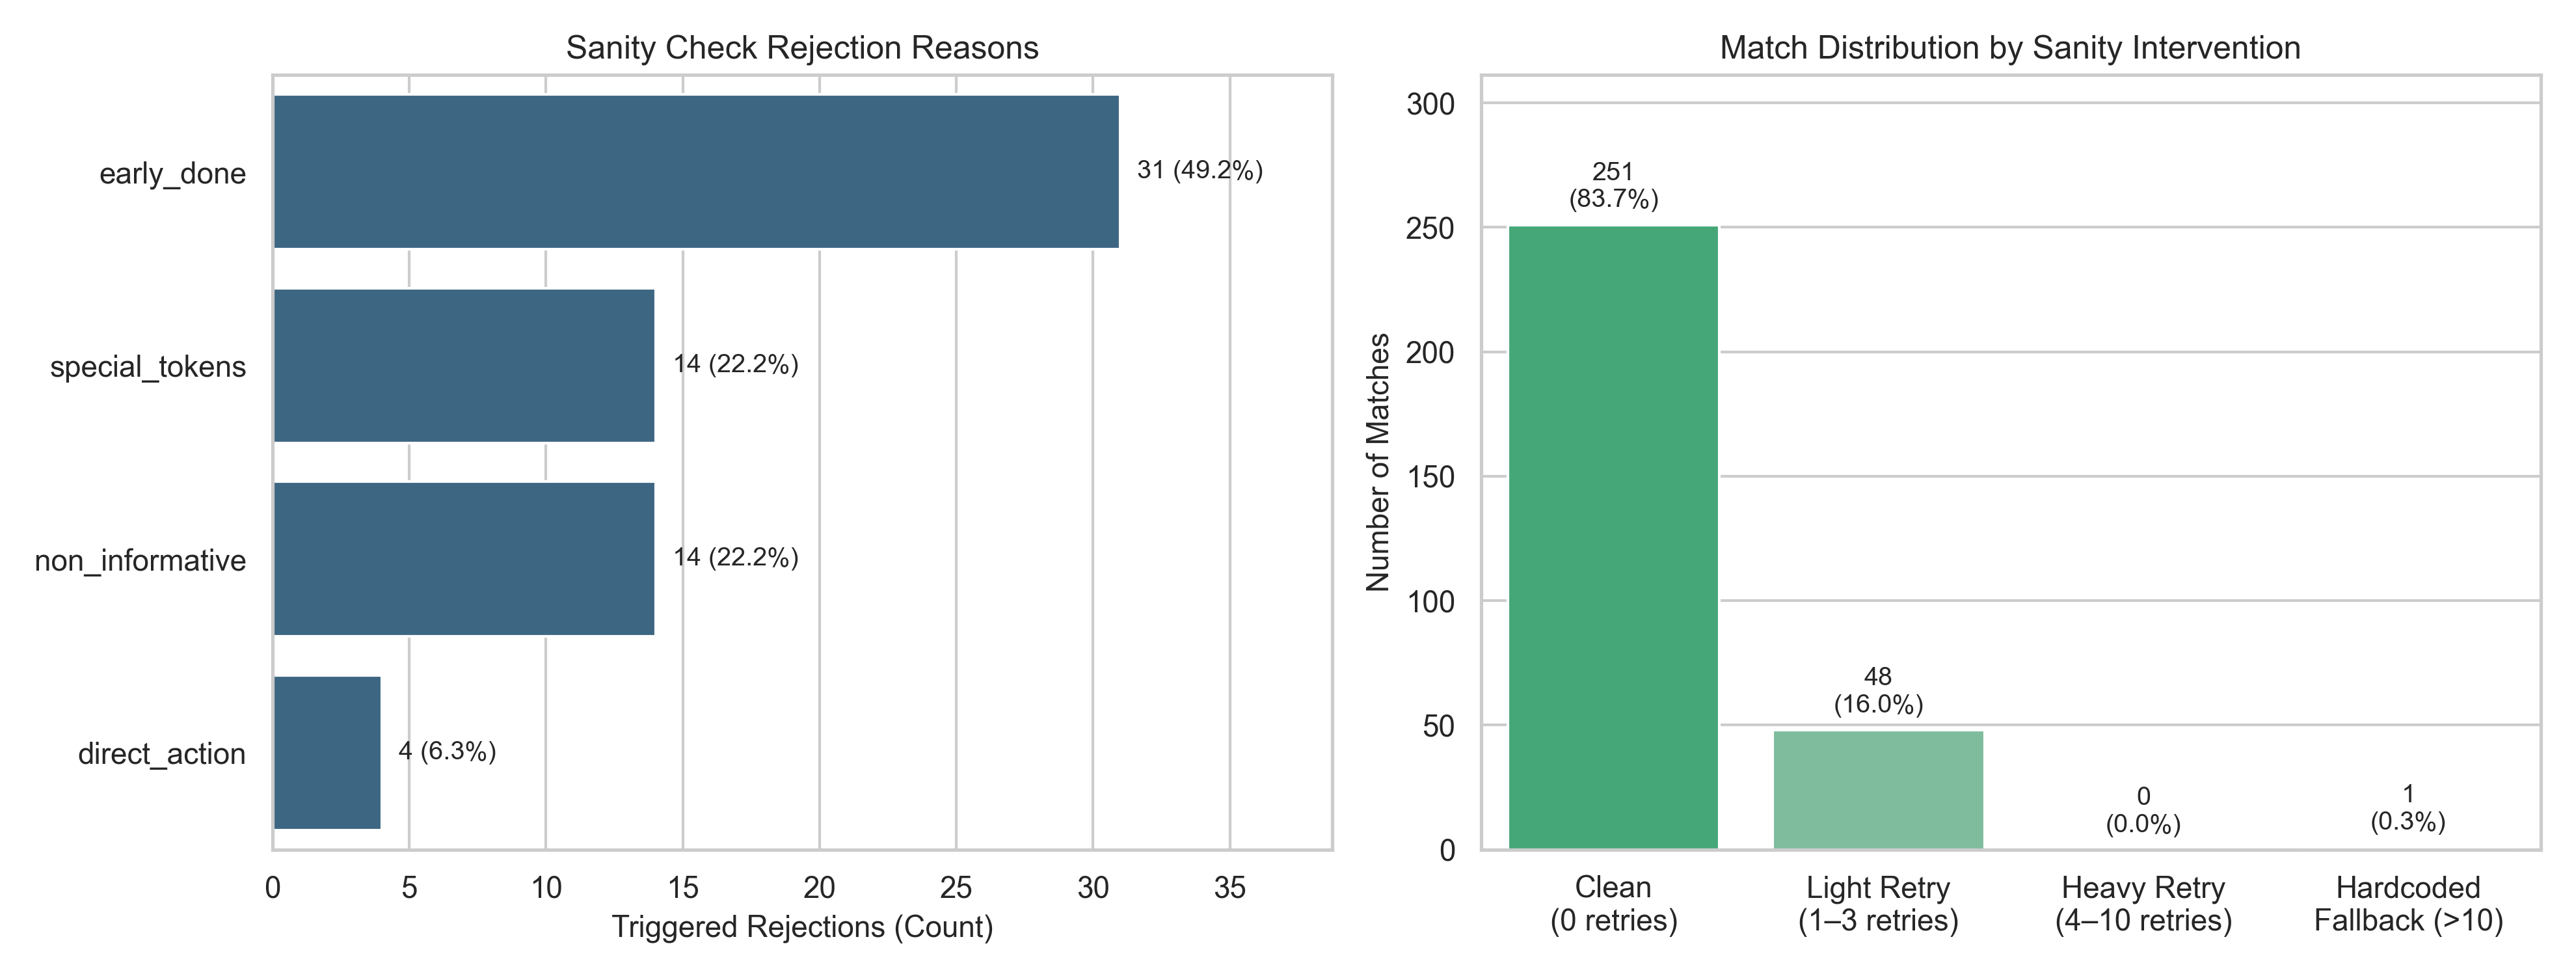
\includegraphics[width=\linewidth]{../reports/sanity_checks_overview.png}
        \end{column}
    \end{columns}
\end{frame}

% ==============================================================================
% SECTION 2: Experimental Results
% ==============================================================================
\section{Experimental Results \& Statistical Analysis}

% SLIDE 6: Primary Result: Baseline vs. Negotiation
\begin{frame}{Primary Result: Baseline vs. Negotiation Ablation}
    \small
    \begin{columns}[T, totalwidth=\textwidth]
        \begin{column}{0.43\textwidth}
            \scriptsize
            \begin{tabular}{lcc}
                \toprule
                \textbf{Metric}       & \textbf{Baseline ($0$)} & \textbf{Chat}                 \\
                \midrule
                Matches (Agents)      & $200$ ($400$)           & $300$ ($600$)                 \\
                Cooperation Rate      & $0.0\%$                 & $\mathbf{63.7\%}$             \\
                $95\%$ Wilson CI      & $[0.0\%, 1.0\%]$        & $[59.7\%, 67.4\%]$            \\
                Mutual Coop. $(C,C)$  & $0.0\%$                 & $\mathbf{54.0\%}$ ($162/300$) \\
                Mutual Defect $(D,D)$ & $100.0\%$               & $26.7\%$ ($80/300$)           \\
                Mean Payoff / Agent   & $1.00$ pts              & $\mathbf{2.37}$ pts           \\
                \bottomrule
            \end{tabular}
            \vspace{0.25cm}
            \small
            \begin{itemize}
                \setlength{\itemsep}{5pt}
                \item \textbf{Pure Nash Baseline:} Without chat, \texttt{gemma4} defects $100\%$ of the time.
                \item \textbf{Causal Shift:} Cheap talk raises cooperation by $+63.7$ pp (Fisher $p < 0.0001$) and payoff by $+137\%$ (Mann-Whitney $p < 0.0001$).
            \end{itemize}
        \end{column}
        \begin{column}{0.54\textwidth}
            \centering
            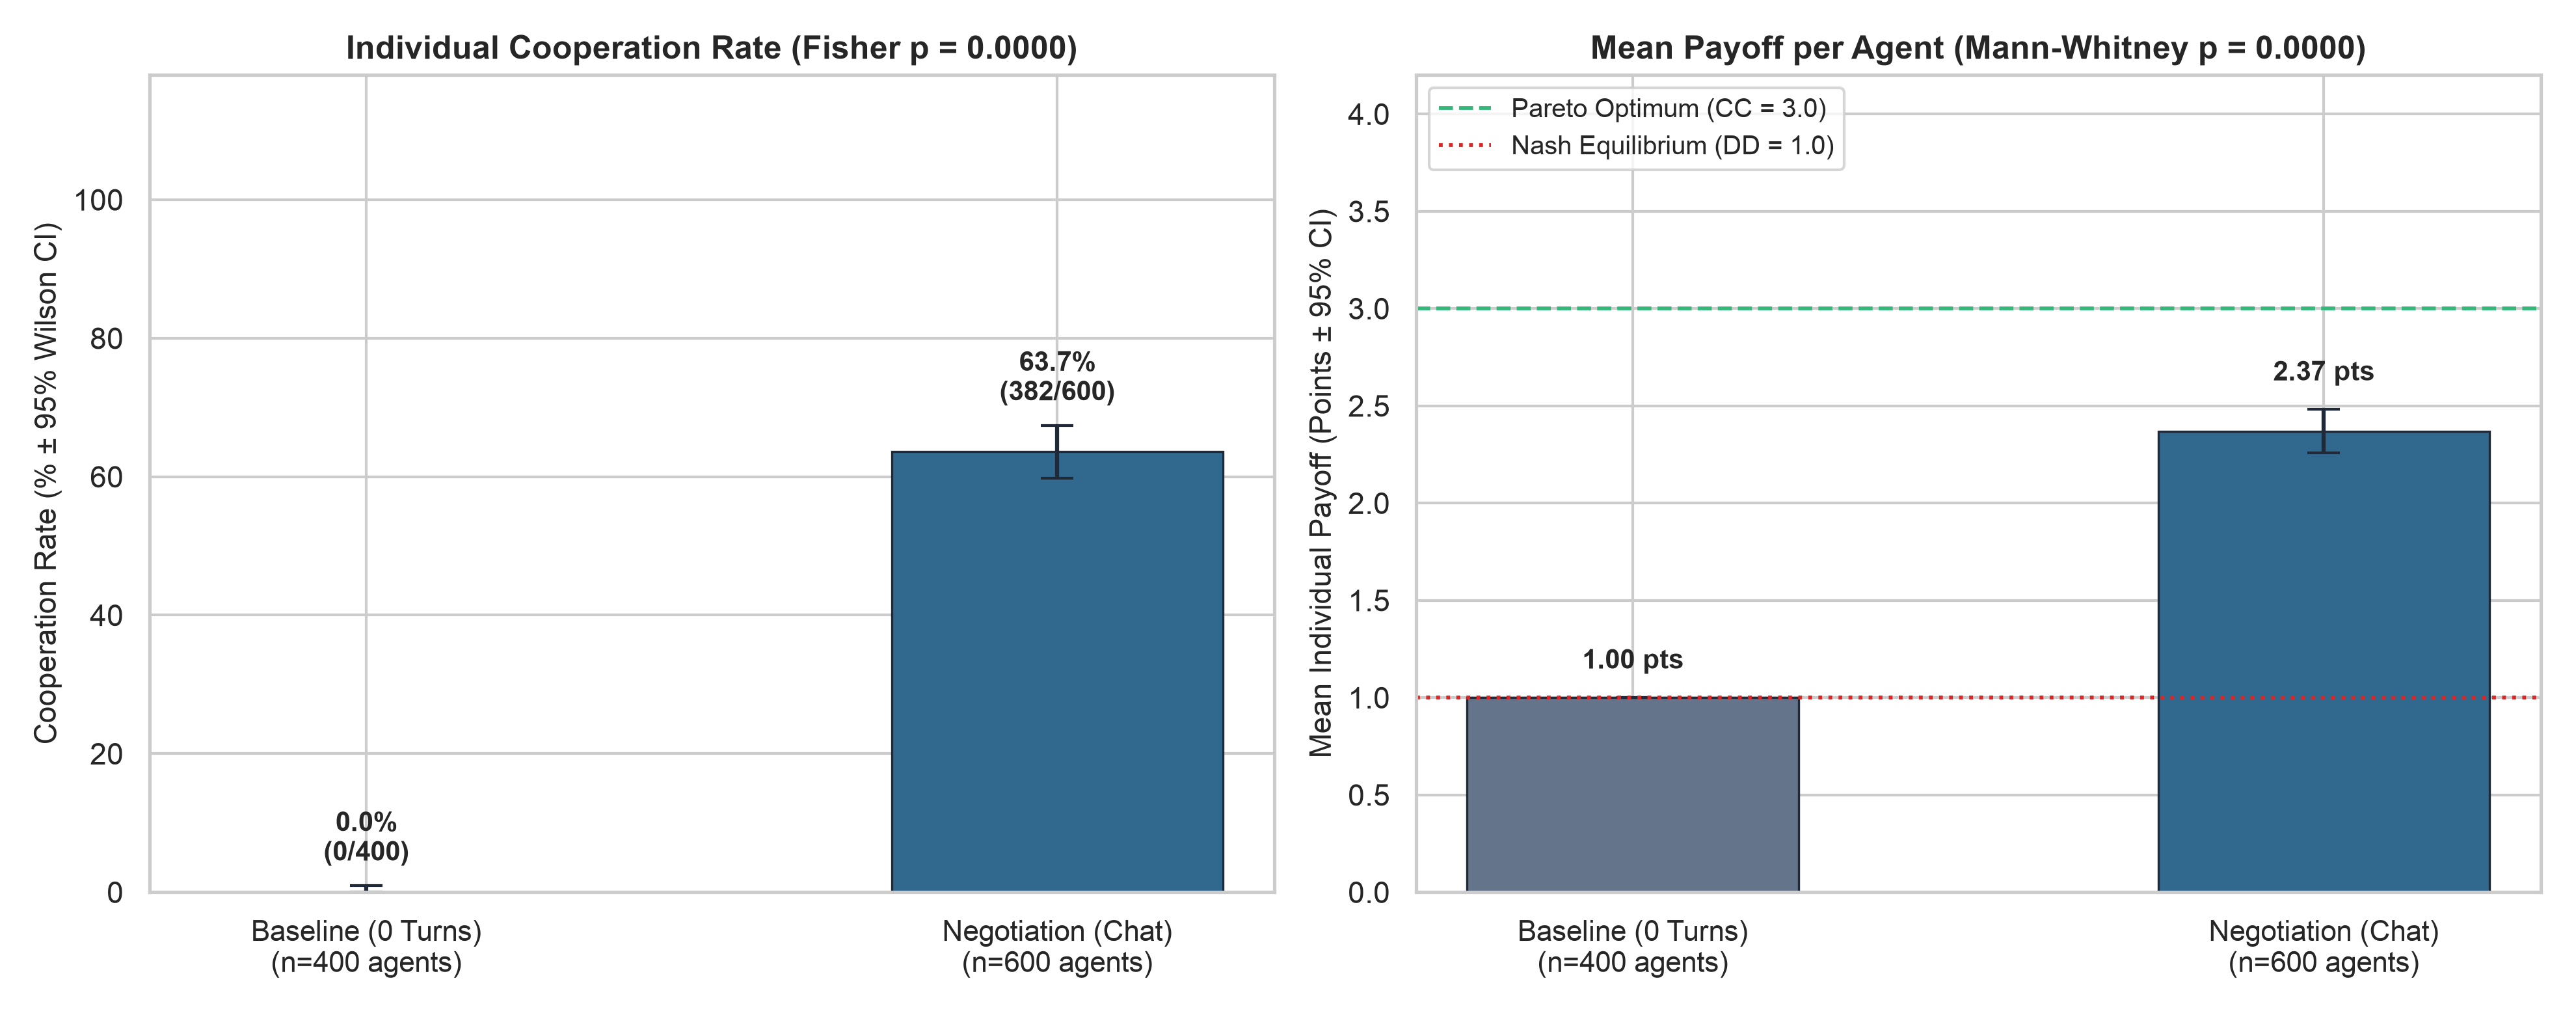
\includegraphics[width=\linewidth]{../reports/baseline/comparison/comparison_cooperation_and_payoff.png}
        \end{column}
    \end{columns}
\end{frame}

% SLIDE 7: Joint Action Distributions & Pairwise Synchronization
\begin{frame}{Joint Action Distributions \& Pairwise Synchronization}
    \small
    \begin{columns}[T, totalwidth=\textwidth]
        \begin{column}{0.43\textwidth}
            \vspace{0.1cm}
            \begin{itemize}
                \setlength{\itemsep}{7pt}
                \item \textbf{Three Emergent Regimes:}
                      \begin{itemize}
                          \item \textbf{Mutual Coop. ($54.0\%$):} Pareto optimal $(3,3)$.
                          \item \textbf{Mutual Defect ($26.7\%$):} Defensive Nash $(1,1)$.
                          \item \textbf{Betrayal ($19.3\%$):} Asymmetric exploitation ($28$ vs. $30$ matches).
                      \end{itemize}
                \item \textbf{Intra-Dialogue Synchronization:} Given marginal cooperation $p = 0.637$, independent pairing yields symmetric outcomes in only $p^2 + (1-p)^2 = 53.7\%$.
                \item Empirically, symmetric outcomes $(C,C)$ and $(D,D)$ reach \textbf{$80.7\%$} ($\chi^2 = 101.68, p < 10^{-23}$).
            \end{itemize}
        \end{column}
        \begin{column}{0.53\textwidth}
            \centering
            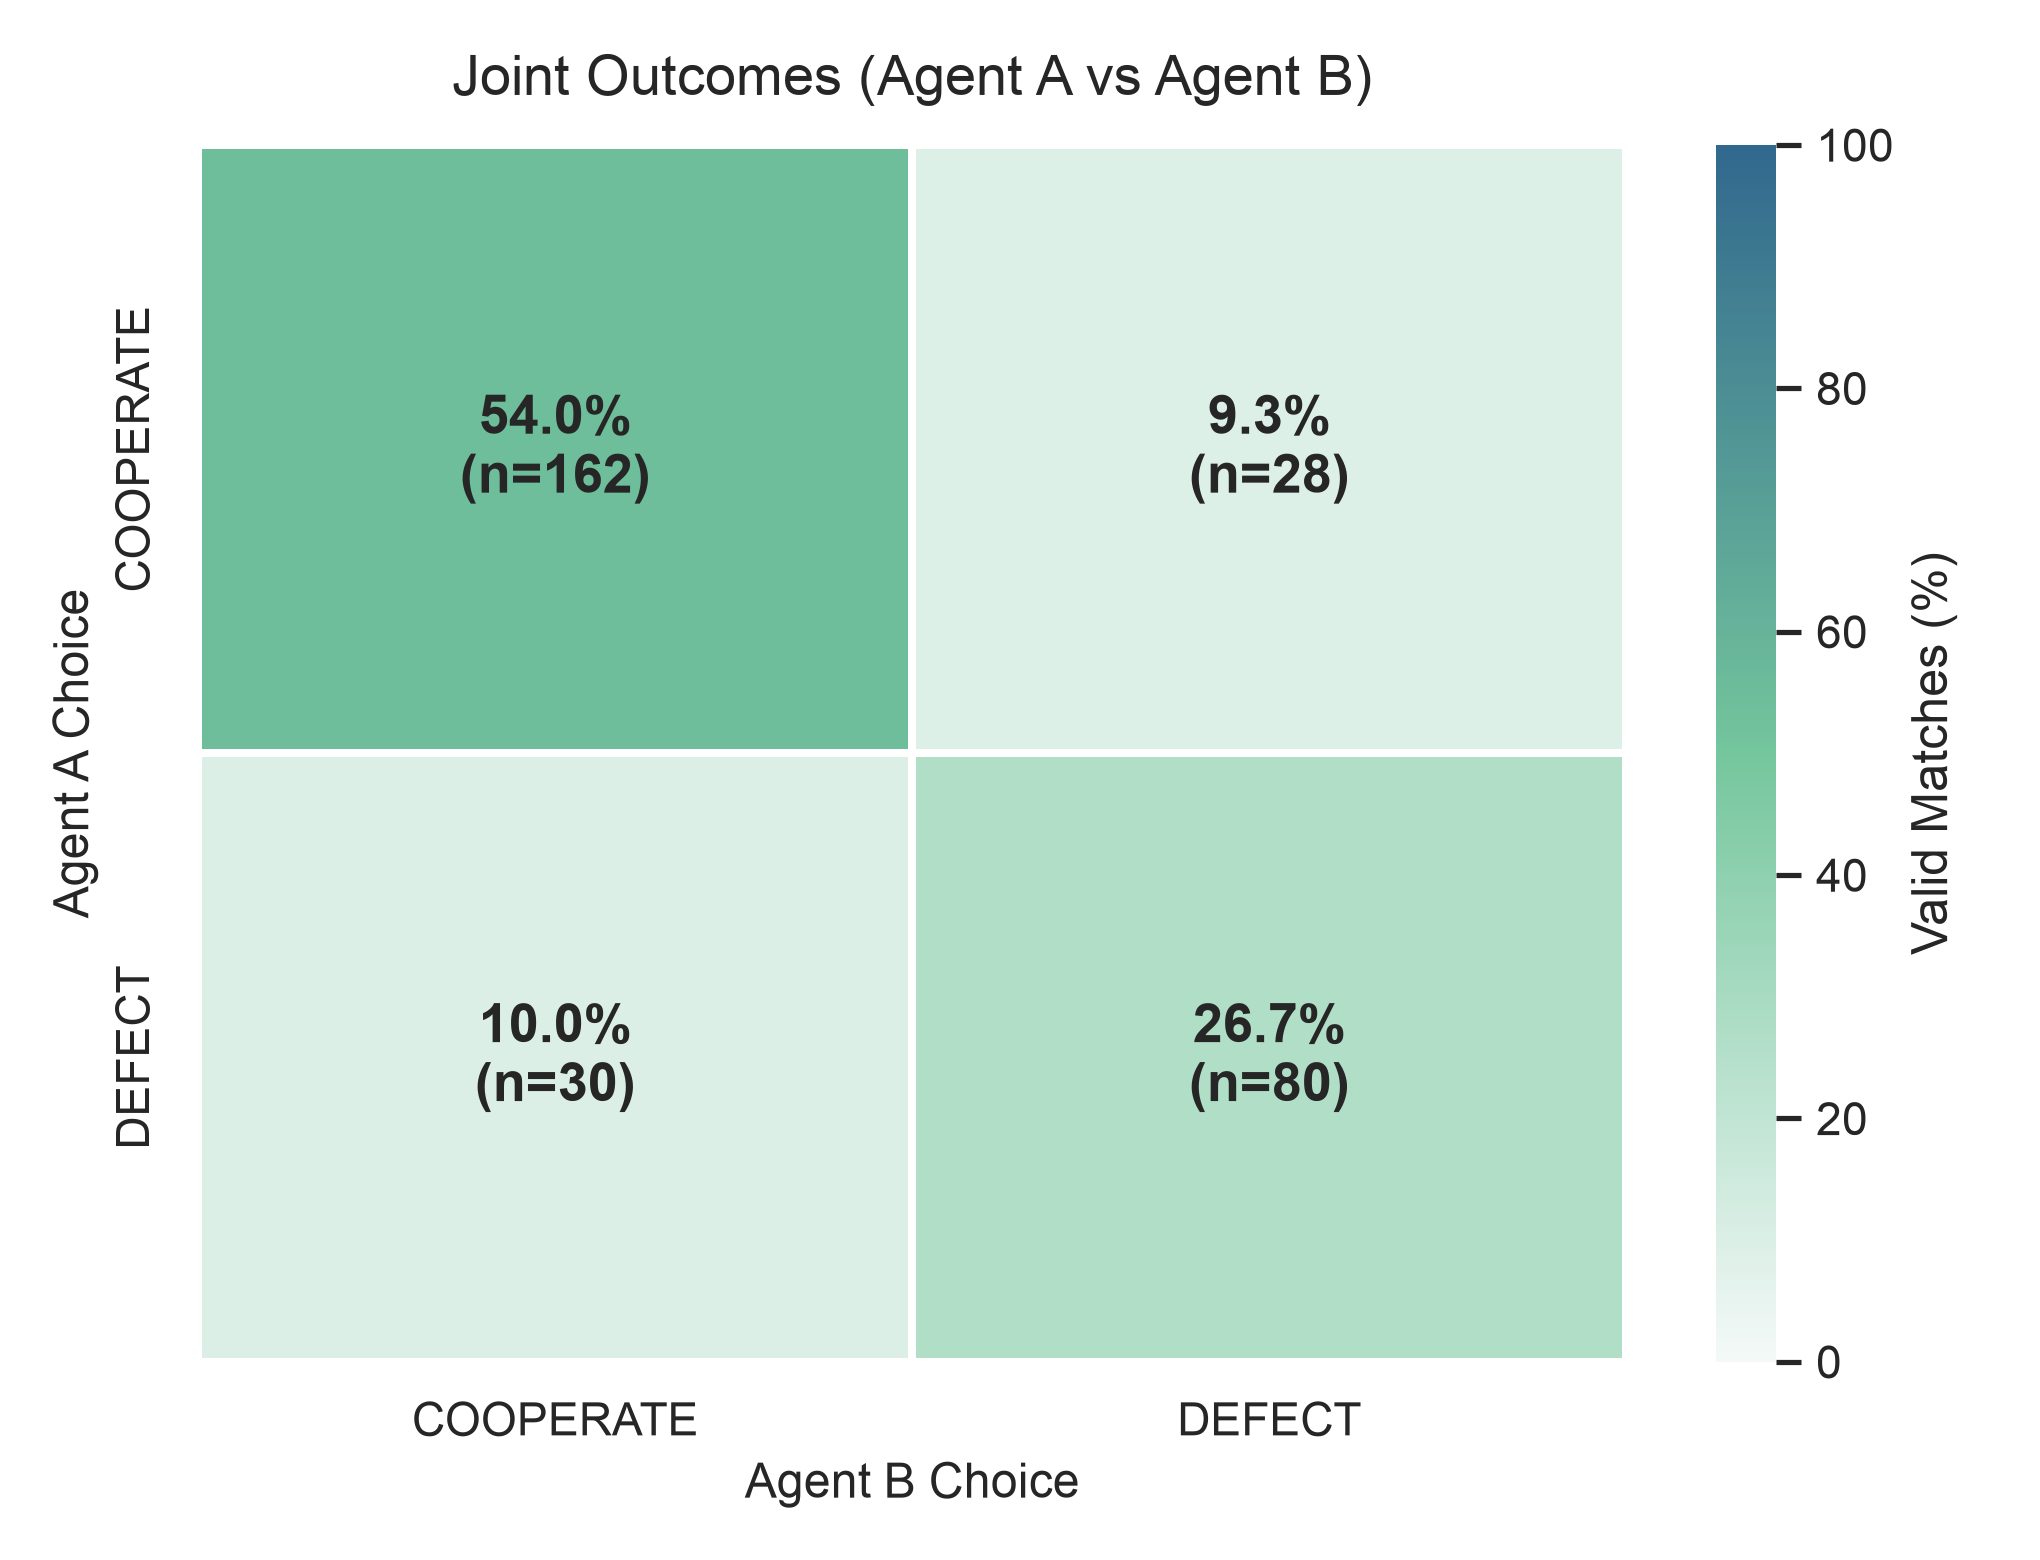
\includegraphics[width=\linewidth]{../reports/outcome_matrix_heatmap.png}
        \end{column}
    \end{columns}
\end{frame}

% SLIDE 8: Economic Payoffs & Symmetry Controls
\begin{frame}{Economic Payoffs \& Structural Symmetry Controls}
    \small
    \begin{columns}[T, totalwidth=\textwidth]
        \begin{column}{0.48\textwidth}
            \textbf{Mean Payoff by Strategy (With Chat)}
            \vspace{0.2cm}
            \footnotesize
            \begin{tabular}{lcc}
                \toprule
                \textbf{Strategy}  & \textbf{Player A} & \textbf{Player B} \\
                \midrule
                \textbf{Cooperate} & $2.56 \pm 1.07$   & $2.53 \pm 1.09$   \\
                \textbf{Defect}    & $2.09 \pm 1.79$   & $2.04 \pm 1.76$   \\
                \bottomrule
            \end{tabular}
            \vspace{0.25cm}
            \small
            \begin{itemize}
                \setlength{\itemsep}{6pt}
                \item \textbf{Payoff Inversion:} Mean payoff for \texttt{COOPERATE} ($2.55$ pts) significantly exceeds \texttt{DEFECT} ($2.06$ pts).
                \item \textbf{Mann-Whitney $U$ Test:} $U = 51840.0$ ($p < 0.0001$) --- negotiation makes cooperation profitable despite $19.3\%$ betrayal risk.
            \end{itemize}
        \end{column}
        \begin{column}{0.48\textwidth}
            \textbf{Experimental Symmetry Validation}
            \vspace{0.2cm}
            \footnotesize
            \begin{tabular}{lcc}
                \toprule
                \textbf{Hypothesis Test}                       & \textbf{Statistic} & \textbf{$p$-value} \\
                \midrule
                Role (\texttt{A} vs. \texttt{B})               & $\chi^2 = 0.0072$  & $0.9324$           \\
                Speaking Order ($1\text{st}$ vs. $2\text{nd}$) & $\chi^2 = 0.0648$  & $0.7990$           \\
                Exploitation ($30$ vs. $28$)                   & Binomial           & $0.8957$           \\
                \bottomrule
            \end{tabular}
            \vspace{0.25cm}
            \small
            \begin{itemize}
                \setlength{\itemsep}{6pt}
                \item \textbf{No First-Mover Advantage:} Initiator ($63.0\%$ coop.) and Responder ($64.3\%$ coop.) behave symmetrically.
                \item Unilateral exploitation is balanced between roles ($30$ vs. $28$ matches).
            \end{itemize}
        \end{column}
    \end{columns}
\end{frame}

% SLIDE 9: Linguistic Signals & Dialogue Dynamics
\begin{frame}{Linguistic Signals \& Dialogue Dynamics}
    \small
    \begin{columns}[T, totalwidth=\textwidth]
        \begin{column}{0.39\textwidth}
            \vspace{0.15cm}
            \begin{itemize}
                \setlength{\itemsep}{8pt}
                \item \textbf{Rapid Consensual Closure:} $100\%$ of dialogues end via mutual \texttt{[DONE]} in $2.32 \pm 0.47$ exchanges (min $2$, max $3$).
                \item \textbf{Verbosity Predicts Defection:} Point-biserial correlation between \texttt{words\_per\_turn} and \texttt{DEFECT} is $r = 0.1685$ ($p = 0.0001$) --- longer persuasive turns signal deceptive intent.
                \item \textbf{\texttt{[DONE]} Density:} Cooperators emit higher \texttt{[DONE]} density per $100$ words ($U = 51621.5, p < 0.0001$).
            \end{itemize}
        \end{column}
        \begin{column}{0.58\textwidth}
            \centering
            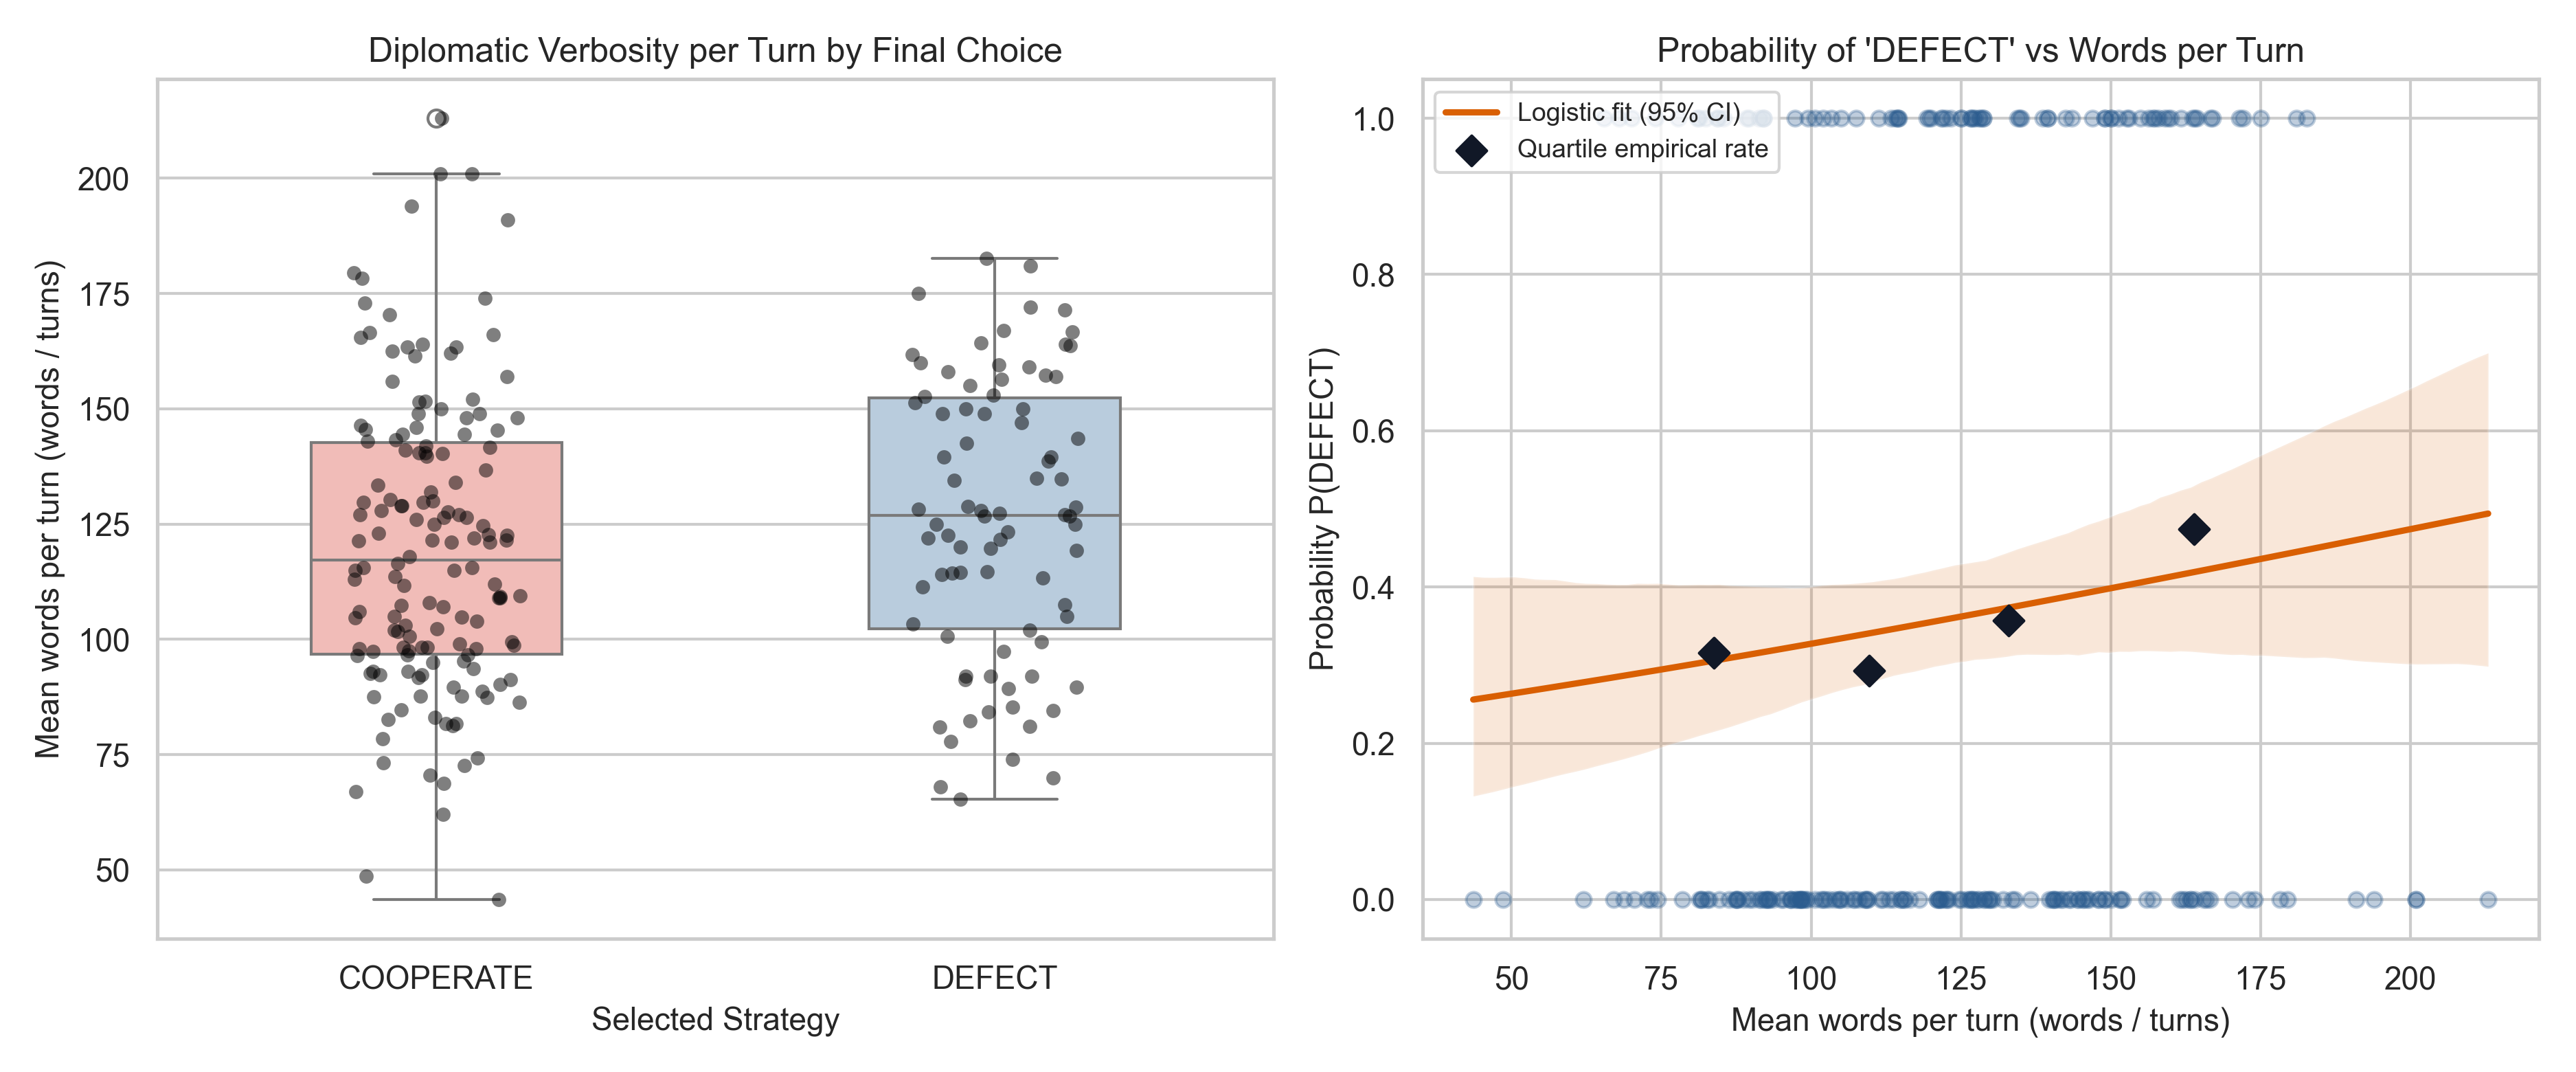
\includegraphics[width=\linewidth]{../reports/verbosity_vs_strategy.png}
        \end{column}
    \end{columns}
\end{frame}

% SLIDE 10: Qualitative Taxonomy of Post-Game Explanations
\begin{frame}{Qualitative Synthesis of Post-Game Explanations}
    \small Map-reduce LLM synthesis across all $600$ post-decision JSON explanations reveals three distinct cognitive frames:
    \vspace{0.2cm}
    \footnotesize
    \begin{tabular}{p{2.9cm}cp{8.6cm}}
        \toprule
        \textbf{Outcome Category}       & \textbf{Count} & \textbf{Dominant Reasoning Pattern}                                                                                                                                           \\
        \midrule
        \textbf{Mutual Cooperators}     & $324$          & \textbf{Contextual Override \& Commitment Device:} Acknowledge $T=5$ temptation, but treat the verbal agreement as a binding social contract securing Pareto utility $(3,3)$. \\
        \addlinespace[4pt]
        \textbf{Mutual Defectors}       & $160$          & \textbf{Defensive Hedging:} Interpret opponent skepticism in chat as strategic risk; fall back to the dominant strategy to guarantee the $1$-pt floor and avoid $0$.          \\
        \addlinespace[4pt]
        \textbf{Exploitative Defectors} & $58$           & \textbf{Calculated Trivialization:} Acknowledge partner's cooperative commitment, then subordinate the social pledge to strict utility maximization ($5 > 3$).                \\
        \bottomrule
    \end{tabular}
    \vspace{0.2cm}
    \scriptsize\color{SoftSlate} Note: Exploited cooperators ($n = 58$) exhibit the same commitment-adherence reasoning as mutual cooperators, honoring the verbal agreement despite partner defection.
\end{frame}

% ==============================================================================
% SECTION 3: Limitations & Conclusion
% ==============================================================================
\section{Limitations, Future Directions \& Conclusion}

% SLIDE 11: Limitations, Future Work & Conclusion
\begin{frame}{Limitations, Future Directions \& Conclusion}
    \small
    \begin{columns}[T, totalwidth=\textwidth]
        \begin{column}{0.48\textwidth}
            \begin{alertblock}{Limitations \& Future Directions}
                \begin{itemize}
                    \setlength{\itemsep}{6pt}
                    \item \textbf{Prompt Sensitivity:} Evaluate diverse initial system framings and persona/incentive perturbations.
                    \item \textbf{Cross-Model Play:} Benchmark asymmetric pairings across heterogeneous LLM families.
                    \item \textbf{Repeated Games:} Introduce multi-round memory and persistent reputation tracking.
                    \item \textbf{Multi-Party Topologies:} Scale negotiation to $N > 2$ group social dilemmas and norm emergence.
                \end{itemize}
            \end{alertblock}
        \end{column}
        \begin{column}{0.48\textwidth}
            \begin{block}{Key Takeaways}
                \begin{itemize}
                    \setlength{\itemsep}{6pt}
                    \item Without communication, \texttt{gemma4} plays the exact Nash Equilibrium ($100\%$ mutual defection).
                    \item Pre-play cheap talk shifts $54.0\%$ of matches to Pareto-optimal cooperation and raises mean payoff from $1.00$ to $2.37$ pts.
                    \item Deception persists ($19.3\%$) and leaves measurable linguistic traces (higher verbosity).
                \end{itemize}
            \end{block}
        \end{column}
    \end{columns}
    \vspace{0.35cm}
    \centering
    \scriptsize\color{SoftSlate}\texttt{\url{https://github.com/GabrieleGranzotto/Multi-Agent-Language-Model-Cooperation-Analysis}}
\end{frame}

\end{document}
